\documentclass[11pt,a4paper]{article}
\usepackage{tikz}
\usetikzlibrary{arrows.meta,positioning}
\usepackage{tabularx}
\usepackage{amsmath,amssymb,amsthm}
\usepackage{geometry}
\geometry{margin=1in}
\usepackage{hyperref}
\usepackage{graphicx}
\usepackage{setspace}
\onehalfspacing

\title{\textbf{Paper A-13: Tectonics, Seismicity, and Volcanism:\\ A Constraint-Driven Flux Dynamics (CDFD) Perspective}}
\author{Steve Bico Mujjabi, MD\\
\small Independent Researcher\\
\small Founder, Vura Labs\\
\small Kampala, Uganda\\
\small ORCID: 0009-0001-0556-5516}
\date{August 2026}

\begin{document}
\maketitle

% BEGIN SHARED-METHODS POINTER
\noindent\textit{Shared Part IV notation and evidence boundaries are defined in \path{PART_IV_METHODS_AND_CLAIM_BOUNDARY.md}. This paper states only its local observables, comparison, and failure conditions.}
% END SHARED-METHODS POINTER


\begin{abstract}
This paper develops a falsifiable CDFD/AFL model of Earth Plate Tectonics. It maps mantle heat, buoyancy, slab pull, ridge push, and stress transfer to driving flux $\Phi$, lithospheric strength, friction, geometry, and phase boundaries to active constraint $C$, fault redistribution, ductile flow, melting, and plate reorganization to responsiveness $S$, and inherited faults, thermal history, compositional structure, and prior strain to structural memory $M_s$. The target outcome is deformation, seismicity, volcanism, and tectonic reorganization, tested against geodesy, seismicity, tomography, heat flow, structural geology, and paleomagnetism. The paper treats universality as a shared model architecture rather than an assertion that unlike systems have the same material mechanism. It states the negative result that would make the mapping unnecessary and places the domain claim inside the cumulative CDFD programme and its reproducible runtime boundary.
\end{abstract}
% BEGIN CONSOLIDATION SCOPE
\section*{Consolidation Scope and Provenance}
This consolidated paper incorporates the plate-tectonic, seismicity, and volcanology scopes formerly carried by Papers A-13, A-14, and D-03. Earthquake occurrence and eruption behaviour remain separate outcomes with separate geophysical baselines and falsifiers.
% END CONSOLIDATION SCOPE


\section{Introduction}

The Earth's crust is not static; it is a continuously evolving mosaic of rigid plates floating atop a viscous, convecting mantle. Where these plates meet, immense stress accumulates along fault zones. Earthquakes occur when the accumulated stress exceeds the frictional strength of the fault, resulting in a sudden, violent displacement.

In CDFD, tectonic fault lines are not merely mechanical interfaces; they are dynamic regulatory constraints across a massive thermodynamic network. Like a clogged biological artery or a bottlenecked supply chain, a locked fault is a system struggling to process its requisite throughput.

\section{The Tectonic Adaptive Surface}
We govern the fault mechanics using the Adaptive Operating Ratio:
\begin{equation}
    \Psi_s = \left( \frac{\Phi}{C} \right) \cdot S \cdot M_s
\end{equation}

In the context of plate boundaries:
\begin{itemize}
    \item \textbf{Flux ($\Phi$)}: The continuous kinetic driving force generated by mantle convection and slab pull pushing the tectonic plates together or past one another.
    \item \textbf{Constraint ($C$)}: The frictional resistance of the fault line, specifically the interlocking rock asperities that prevent smooth sliding.
    \item \textbf{Responsiveness ($S$)}: The elastic capacity of the surrounding crust to deform and absorb stress without breaking.
    \item \textbf{Memory ($M_s$)}: Fault locking. As the fault remains stationary over centuries, chemical bonding and mechanical interlocking fuse the rock faces together. The fault "remembers" its static position, driving $M_s \to 1.0$ and cementing the constraint.
\end{itemize}

\subsection{The Seismic Cycle as a Regime Shift}
During the interseismic period, the tectonic flux ($\Phi$) continues unceasingly from the mantle. However, because the fault is locked by its memory ($M_s$) and friction ($C$), the physical flow of the crust halts at the boundary. The system enters a state of extreme localized constraint ($\Psi_s \ll 1$).

To avoid total stagnation, the system's responsiveness ($S$) flexes: the crust elastically bends, storing the incoming flux $\Phi$ as potential energy. Over decades, this elastic capacity $S$ approaches its ultimate physical limit (the yield strength of the rock).

When $S$ saturates, the adaptive ratio crashes. The system can no longer sustain the incoming flux. The stored topological tension causes a sudden, catastrophic failure of the memory term $M_s$. The interlocking asperities snap. The constraint $C$ instantly drops to near zero (dynamic sliding friction), and the stored potential energy violently converts back into kinetic flux $\Phi$---an earthquake.



\section{Measurement Layer}

% BEGIN PART IV MAJOR CROSS-DOMAIN UPGRADE
\section{Cross-Domain Model Upgrade: Mechanism, Scale, and Tests}

\subsection{Observable Translation}

The paper-specific translation begins with an observable chain rather than a
verbal analogy. For Earth Plate Tectonics, the proposed drive is mantle heat, buoyancy, slab pull, ridge push, and stress transfer.
The active limitation is lithospheric strength, friction, geometry, and phase boundaries. Responsiveness is carried by
fault redistribution, ductile flow, melting, and plate reorganization, while retained state is represented by
inherited faults, thermal history, compositional structure, and prior strain. The outcome to explain is deformation, seismicity, volcanism, and tectonic reorganization.

\begin{table}[htbp]
\centering
\small
\caption{Operational CDFD/AFL map for Paper A-13.}
\begin{tabularx}{\textwidth}{|l|X|X|}
\hline
\textbf{Term} & \textbf{Paper-specific observable meaning} & \textbf{Measurement question} \\
\hline
$\Phi$ & mantle heat, buoyancy, slab pull, ridge push, and stress transfer & What rate, load, gradient, or demand enters the focal system? \\
\hline
$C$ & lithospheric strength, friction, geometry, and phase boundaries & Which measured bottleneck limits transfer, function, or recovery? \\
\hline
$S$ & fault redistribution, ductile flow, melting, and plate reorganization & Which process changes effective capacity or reroutes the load? \\
\hline
$M_s$ & inherited faults, thermal history, compositional structure, and prior strain & Which retained state makes equal present loads produce different futures? \\
\hline
$Y$ & deformation, seismicity, volcanism, and tectonic reorganization & Which outcome is predicted out of sample, with uncertainty? \\
\hline
\end{tabularx}
\end{table}

\begin{figure}[htbp]
\centering
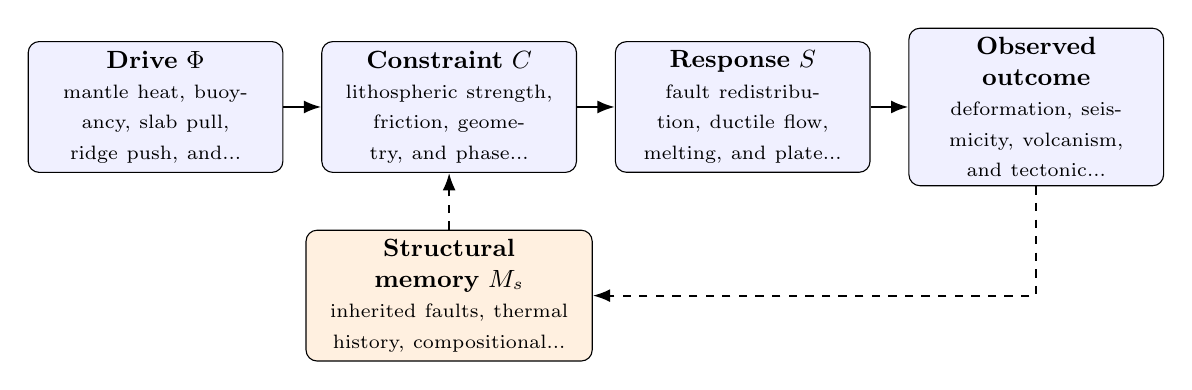
\begin{tikzpicture}[
    node distance=0.48cm,
    every node/.style={font=\small},
    box/.style={draw, rounded corners, align=center, minimum height=1.45cm, text width=3.0cm, fill=blue!6},
    memory/.style={draw, rounded corners, align=center, minimum height=1.25cm, text width=3.4cm, fill=orange!12},
    flow/.style={-{Latex[length=2.2mm]}, thick},
    feedback/.style={-{Latex[length=2.2mm]}, thick, dashed}
]
\node[box] (drive) {\textbf{Drive $\Phi$}\\\scriptsize mantle heat, buoyancy, slab pull, ridge push, and...};
\node[box, right=of drive] (constraint) {\textbf{Constraint $C$}\\\scriptsize lithospheric strength, friction, geometry, and phase...};
\node[box, right=of constraint] (response) {\textbf{Response $S$}\\\scriptsize fault redistribution, ductile flow, melting, and plate...};
\node[box, right=of response] (outcome) {\textbf{Observed outcome}\\\scriptsize deformation, seismicity, volcanism, and tectonic...};
\node[memory, below=0.72cm of constraint] (memory) {\textbf{Structural memory $M_s$}\\\scriptsize inherited faults, thermal history, compositional...};
\draw[flow] (drive) -- (constraint);
\draw[flow] (constraint) -- (response);
\draw[flow] (response) -- (outcome);
\draw[feedback] (outcome.south) |- (memory.east);
\draw[feedback] (memory.north) -- (constraint.south);
\end{tikzpicture}
\caption{Paper A-13 observable CDFD/AFL architecture for Earth Plate Tectonics. Solid arrows give the proposed forward chain; dashed arrows make history-dependent feedback explicit.}
\label{fig:a13-architecture}
\end{figure}

\subsection{Paper-Specific Causal Hypothesis}

For this paper, the hypothesized causal sequence is specific. A change in
mantle heat, buoyancy, slab pull, ridge push, and stress transfer arrives faster than fault redistribution, ductile flow, melting, and plate reorganization can compensate.
This raises or redistributes lithospheric strength, friction, geometry, and phase boundaries. If the load persists,
the retained state encoded by inherited faults, thermal history, compositional structure, and prior strain changes the next response, so a later event of equal
magnitude can produce a different trajectory in deformation, seismicity, volcanism, and tectonic reorganization. The
scientific task is to estimate that sequence against the best ordinary model of
the domain, not merely to redescribe the outcome after it occurs.

\subsection{Cross-Scale Translation Without Mechanistic Erasure}

For the Earth systems family, the cross-domain translation compares coupled transport, finite environmental capacity, buffering, and retained landscape or ecosystem state. It cannot erase conservation laws, geometry, or scale; it must expose where those domain equations create comparable overload and recovery structures. \cite{Holling1973,Turing1952,BakTangWiesenfeld1987}
The required scale declaration for this paper is seconds to hundreds of millions of years; grains to plates. At short
scales, the key question is whether the incoming drive is transmitted,
buffered, or diverted. At intermediate scales, response changes effective
capacity and network exposure. At long scales, retained structure can alter the
state space itself. A result is genuinely cross-scale only when the aggregation
rule is stated and the same conclusion is not an artifact of averaging.

\subsection{Evidence Ladder and Discriminating Tests}

\begin{table}[htbp]
\centering
\small
\caption{Evidence ladder for Paper A-13. Each rung can fail independently.}
\begin{tabularx}{\textwidth}{|p{0.17\textwidth}|X|X|}
\hline
\textbf{Test} & \textbf{Design} & \textbf{Discriminating result} \\
\hline
Proxy audit & Measure geodesy, seismicity, tomography, heat flow, structural geology, and paleomagnetism and preregister how each record maps to $\Phi$, $C$, $S$, $M_s$, and $Y$. & The mapping fails if proxies are non-identifiable, circular, or change meaning across cases. \\
\hline
Load ramp & Apply or observe a stress-transfer sequence across a mapped fault network while estimating the dominant constraint and response time. & A threshold claim requires a reproducible nonlinear change and uncertainty bounds, not a visually chosen breakpoint. \\
\hline
Recovery and memory & Match present load across units with different histories, then compare recovery paths. & The memory claim requires history-dependent divergence after current conditions are controlled. \\
\hline
Model comparison & Compare the baseline domain model with and without the CDFD/AFL state variables using held-out data. & The paper's stated falsifier is: explicit memory and network terms do not improve forecasts or retrospective explanation. \\
\hline
\end{tabularx}
\end{table}

\subsection{Research Programme and Boundary Conditions}

The immediate research programme has four steps. First, construct a documented
dataset from geodesy, seismicity, tomography, heat flow, structural geology, and paleomagnetism and retain raw units before normalization.
Second, fit a baseline domain model and report its calibration and out-of-sample
error. Third, add the smallest identifiable CDFD/AFL state extension and test
whether it improves prediction of deformation, seismicity, volcanism, and tectonic reorganization. Fourth, repeat the
analysis across the declared scale range and publish negative cases as part of
the cross-domain translation audit.

% END PART IV MAJOR CROSS-DOMAIN UPGRADE

\section{Conclusion}
Earthquakes are formally comparable at the declared-variable level to stellar core collapse or metabolic phase shifts. They represent the abrupt topological resetting of an over-constrained system forced to shed its chronic memory to restore a sustainable flow regime. By applying CDFD, seismology transitions from a descriptive science of elastic rebound into a universal thermodynamic physics.
\section*{Conflict of Interest} The author declares no conflict of interest.
\section*{Data Availability}
Part-specific runtime diagnostics are under each Part's \path{outputs/} directory.

Release-wide code: \path{Part_E_Synthesis/supplementary/}.

Generated summaries: \path{Part_E_Synthesis/outputs/}.

Figures: \path{Part_E_Synthesis/figures/}.


\section{Reference Layer}
\bibliographystyle{plain}
\bibliography{universal_afl_references}
\end{document}
